\documentclass[a4paper, 10pt, twocolumn]{article}

\usepackage[T1]{fontenc}
\usepackage[utf8]{inputenc}
\usepackage[left=1.8cm, top=1.8cm, total={18cm, 25cm}]{geometry}
\usepackage[unicode]{hyperref}
\usepackage[slovak]{babel}
\usepackage{enumitem}
\usepackage{graphicx}

\title{Implementačná dokumentácia k~2.~úlohe do IPP 2020/2021}
\author{Meno a~priezvisko: Jakub Bartko \\ Login: xbartk07}
\date{}

\begin{document}
\maketitle

\section{Interprét}
    Interprét popísaný v~tejto dokumentácií napísaný v~jazyku Python~3.8 slúži na interpretáciu XML reprezentácie kódu \texttt{IPPcode21}.
    
    \subsection{Činnosť}\label{sub:cinnost}
        Činnosť skriptu \texttt{interpret.py} je možné rozdeliť na spracovanie argumentov príkazového riadka, načítanie XML reprezentácie zdrojového kódu, lexikálnu a~syntaktickú analýzu inštrukcií a~argumentov, ich vykonávanie, generovanie výstupov a~zbieranie štatistík o~týchto inštrukciách.
        
        Na základe argumentov príkazového riadka sa získa XML reprezentácia, ktorá je prevedená na stromovú štruktúru s~využitím modulu \texttt{xml.etree.ElementTree}. Po kontrole koreňového prvku sú inštrukcie zoradené podľa atribútu \texttt{order} a~skontroľujú sa ich tagy, atribúty a~počet a~formát argumentov. 
        
        \label{sub:label}V rámci tejto kontroly sa predom definujú cieľové návestia a~inštrukcie \texttt{LABEL} sú ďalej ignorované.
        
        Ďalej sú iterované objekty jednotlivých inštrukcií. Podľa ich operačného kódu sa zavolá príslušná obslužná funkcia, získajú a~skontrolujú sa argumenty (v~stromovej štruktúre potomkovia objektu inštrukcie) a~vykoná sa vnútorná funkcionalita danej inštrukcie.
    
    \subsection{Štruktúra kódu a~implementácia}\label{sub:struct}
        Funkcie na získavanie a~kontrolu argumentov, obsluhu inštrukcií a~riadenie toku programu a~pomocné štruktúry využívané na sémantickú analýzu a~zbieranie štatistík sú súčasťou triedy \texttt{Interpret}. Činnosť metód tejto triedy je možné rozdeliť na niekoľko kategórií.
        
        \textbf{Argumenty inštrukcií} sú na základe daného objektu inštrukcie a~poradia argumentu získavané funkciou \texttt{get\_arg}. Podľa definovaného typu argumentu, t.~j.~\texttt{var}, \texttt{symb}, \texttt{label} alebo \texttt{type}, sa skontrolujú jeho atribúty a~text a~vráti sa spracovaný argument nasledovne:
        \begin{itemize}[noitemsep,topsep=2pt]
            \item \texttt{var} - názov rámca a~premennej,
            \item \texttt{symb} - typ a~hodnota premennej alebo konštanty,
            \item \texttt{label} - názov návestia,
            \item \texttt{type} - objekt enumerátora \texttt{Type}.
        \end{itemize} \smallskip
        
        Funkcie na \textbf{prácu s~premennými} využívajú asociatívny zoznam obsahujúci globálny a~dočasný rámec a~zásobník lokálnych rámcov. Každá premenná je reprezentovaná objektom triedy \texttt{Var} uchovávajúcim dvojicu: typ a~hodnota. Na zistenie unikátnosti/výskytu určitej premennej sa využíva funkcia \texttt{is\_unique} a~na uloženie jej typu a~hodnoty do príslušného rámca pod špecifikované meno funkcia \texttt{store}. Jednotlivé rámce sú teda implementované ako asociatívne zoznamy vo formáte \mbox{\textit{názov\_premennej: Var(typ, hodnota)}}.
        
        \textbf{Aritmetické}, \textbf{relačné} a~\textbf{logické operácie} využívajú spoločnú funkciu \texttt{operations}. V~rámci tejto funkcie sa cieľové úložisko a~hodnoty operandov získajú buď z~argumentov inštrukcie, alebo v~prípade koncovky~\uv{\textit{-S}} z~dátového zásobníka (\textit{\underline{S}tack}). Následne sa podľa typu operácie (aritmetická, relačná,~\dots) skontrolujú typy operandov, získa sa jej výsledok využitím asociatívneho zoznamu lambda výrazov a~uloží sa buď do cieľovej premennej alebo na dátový zásobník.
        
        Operácie s~\textbf{dátovým zásobníkom} pracujú nad zoznamom dvojíc (\texttt{tuple}) typov a~hodnôt. V~prípade chýbajúceho argumentu využijú dvojicu na vrchu zásobníka.
        
        Do kategórie \textbf{riadenia toku programu} patrí funkcionalita na spravovanie návestí, vyhodnocovanie podmienených skokov a~výber nasledujúcej inštrukcie v~hlavnej iterácií. Návestia sú definované v~rámci kontroly inštrukcií spomenutej v~kapitole~\ref{sub:cinnost}, t.~j. sú uložené do asociatívneho zoznamu návestí ako \textit{názov:}~\texttt{order}. V~prípade skoku na návestie sa z~tohoto zoznamu získa príslušný \texttt{order} a~jeho hodnota sa vráti do tela iterovania inštrukcií. Ak návratová hodnota zavolanej obslužnej funkcie chýba, iterácia pokračuje inštrukciou na nasledujúcom indexe; v~opačnom prípade sa v~stromovej štruktúre XML reprezentácie nájde inštrukcia s~príslušnou hodnotou argumentu \texttt{order} a~iterácia pokračuje inštrukciou na indexe, ktorý nájdenej inštrukcií nasleduje.
        
        Popisy kategórií inštrukcií neuvedené v~tejto kapitole boli vynechané z~dôvodu triviálnosti ich riešenia a~priamočiarosti implementácie. Ich obsluhu je možné zhrnúť na: získanie cieľovej premennej, získanie hodnôt argumentov a~kontrolu ich typov a~uloženie výsledku, ktorého získanie sa zvyčajne zmestilo do samotnej operácie ukladania.
    
    \subsection{Rozšírenia}
        Rozšírenie \texttt{FLOAT} je implementované ako prídavná funkcionalita obslužných funkcií pre inštrukcie aritmetických, relačných a~logických operácií, inštrukcie načítavania, výpisu atď. Okrem toho sú v~rámci toho rozšírenia implementované funkcie na prevod medzi typmi \texttt{float} a~\texttt{int} (a~ich zásobníkové verzie).
        
        Ako už bolo uvedené v~predchádzajúcej kapitole~\ref{sub:struct}, operandy inštrukcií rozšírenia \texttt{STACK} sú získavané z~dátového zásobníku, na ktorý sa taktiež ukladajú ich výsledky. V~ostatných ohľadoch sú interpretované analogicky so svojimi nezásobníkovými verziami.
        
        Argumenty príkazovej riadky rozšírenia \texttt{STATI} sú spracované spolu so základnými funkciou \texttt{get\_args} a~predané inštancií triedy \texttt{Interpret}. Na sledovanie počtu vykonaných inštrukcií sa využíva vnútorné počítadlo tejto triedy, aktualizované pri zavolaní príslušnej obsluhy prostredníctvom funkcie \texttt{Interpret.run}. Na tomto mieste sa taktiež zväčší hodnota počtu zavolaní aktuálnej inštrukcie v~asociatívnom zozname s~formátom \texttt{order:}~\textit{počet\_zavolaní}, prípadne so doň táto dvojica vloží ako prvý výskyt s~hodnotou~1. Na sledovanie počtu platných inicializovaných premenných sa využívajú počítadlá aktualizované pri zápise hodnoty do premennej funkciou \texttt{Var.set} v~prípade, že jej pôvodná hodnota nie je definovaná, a~pri manipulácií so zásobníkom lokálnych rámcov tak, že v~rámci obsluhy funkcie \dots~sa inicializované premenné:
        \begin{itemize}
            \item \texttt{CREATEFRAME}: zahodeného dočasného rámca \textbf{odčítajú},
            \item \texttt{PUSHFRAME}: prekrytého lokálneho rámca \textbf{odčítajú},
            \item \texttt{POPFRAME}: zahodeného dočasného rámca odčítajú a~inicializované premenné odkrytého lokálneho rámca sa pripočítajú.
        \end{itemize}
        Tieto štatistiky sú na po spracovaní všetkých inštrukcií alebo po zavolaní inštrukcie \texttt{EXIT} zapísané do špecifikovaného súboru.

\section{Testovací skript}
    Skript \texttt{test.php} slúži na testovanie činnosti skriptov \texttt{parse.php} a~\texttt{interpret.py} buď samostatne, alebo ako jednotného funkčného celku.
    
    \subsection{Činnosť a~implementácia}
        Tento skript využíva dve globálne štruktúry: \mbox{\texttt{Handles}\,--\,na} uloženie spracovaných argumentov príkazového riadka a~kontrolu špecifikovaných vstupných súborov; a~štruktúru \texttt{Outputs}, ktorá sa využíva na sledovanie úspešnosti testov a~zápis generovaného HTML výstupu.
        
        Špecifikovaný súbor s~testami môže byť iterovaný rekurzívne, no z~hľadiska implementácia sa od nerekurzívneho prechádzania líši len v~konštrukcií iterátora a~formáte výstupu. Pre každý zdrojový súbor (.src) sa skontrolujú a~v~prípade potreby dogenerujú príslušné referenčné súbory. Ďalej sa zostaví a~zavolá príkaz na základe špecifikovaného testovaného skriptu/, ktorý spustí testované skripty (alebo ich kombináciu) s~príslušným vstupným súborom na vstupe, uloží výstup a~získa návratovú hodnotu.
        
        Daný test potom validuje tak, že porovná získanú a~referenčnú návratovú hodnotu a~v~prípade úspešného ukončenia testovaného skriptu porovná aj získaný výstup s~výstupom referenčným unixovým nástrojom \texttt{diff}, prípadne výstup vo formáte XML nástrojom \texttt{A7Soft JExamXML}. Na záver validácie sa upracú vytvorené dočasné súbory.
    
        Výsledok validácie sa vráti do tela iterácie, kde sa ďalej aktualizujú počítadlá na sledovanie úspešnosti testov a~pripíše sa HTML výstup vygenerovaný pre daný test.
        
        Na záver sa finalizuje generovaný HTML výstup a~vypíše sa na \texttt{STDOUT}. Výstupný výpis (obr.~\ref{fig:output}) pozostáva z~absolútneho a~relatívneho počtu a~interaktívnych zoznamov testov zoskupených podľa úspešnosti.
        
    \begin{figure}
        \centering
        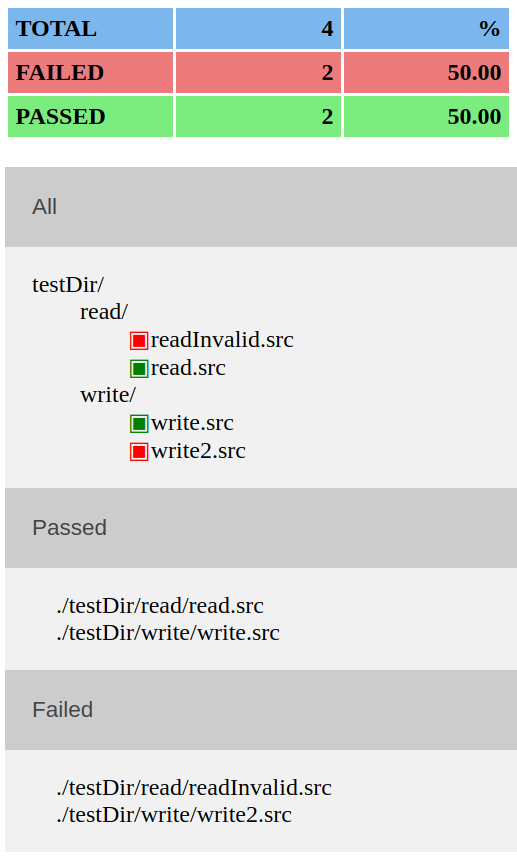
\includegraphics[width=0.48\textwidth]{testExample.png}
        \caption{Ukážka výstupného HTML súboru}
        \label{fig:output}
    \end{figure}

\end{document}
